% To create a slide, use the following:
% \begin{frame}{TITLE}
%     BODY
% \end{frame}


\begin{frame}{Work Done Till Now}
    \begin{itemize}
        \item Front End Design 
        \item Callifier Demo 
    \end{itemize}
\end{frame}


\begin{frame}{Software Devlopment for 2024 Summer}
    \begin{itemize}
        \item Fullstack Devlopment
        \item Auth0/ Mongodb
        \item Security/Networks
        \item Aws Architecture
    \end{itemize}
\end{frame}



\begin{frame}{Resolution Scaling}
    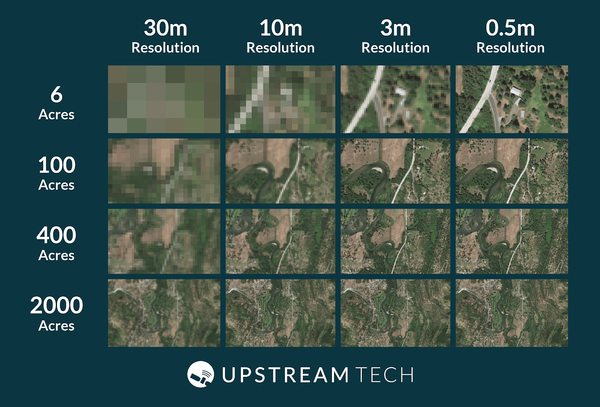
\includegraphics[height=0.5\textheight,width=0.5\textwidth,keepaspectratio]{images/mm_ml/Resolutions.png}
    \begin{enumerate}
        \item Super Resolution CNN 
        \item Generative Upscaling
        \item Adaptive Pooling
    \end{enumerate}
\end{frame}


\begin{frame}{ML Model}
     \begin{itemize}
        \item Foundational models
        \item Visual Transformer vs CNN
    \end{itemize}
    ImageNet objects vs satellite imagery:

    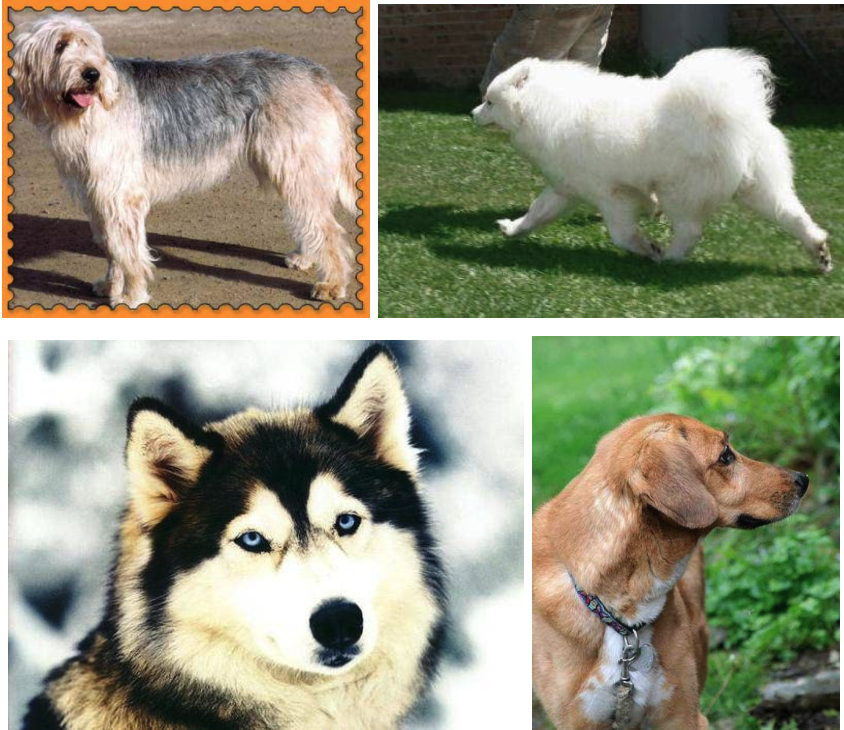
\includegraphics[height=0.35\textheight,width=0.35\textwidth,keepaspectratio]{images/mm_ml/Dogs.png}
    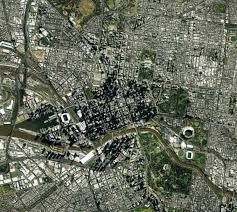
\includegraphics[height=0.35\textheight,width=0.35\textwidth,keepaspectratio]{images/mm_ml/Satellite.jpeg}
   
\end{frame}




% To create a slide with a bullet list, use the following:
% \begin{frame}{TITLE}
%     \begin{itemize}
%         \item ITEM 1
%         \item ITEM 2
%     \end{itemize}    
% \end{frame}

% To create a slide with numbered list, use the following:
% \begin{frame}{TITLE}
%     \begin{enumerate}
%         \item ITEM 1
%         \item ITEM 2
%     \end{enumerate}
% \end{frame}

% To create a slide with a graphic:
% 1. Add the graphic to this folder (named picture.png)
% 2. Use the following:
% \begin{frame}{TITLE}
%     \centering
%     \includegraphics[height=0.7\textheight,width=0.7\textwidth,keepaspectratio]{picture.png}
% \end{frame}

% To create a slide with two columns, use the following:
% \begin{frame}{TITLE}
%     \begin{columns}
%         \begin{column}{0.5\textwidth}
%             COLUMN 1 BODY
%         \end{column}
%         \begin{column}{0.5\textwidth}
%             COLUMN 2 BODY
%         \end{column}
%     \end{columns}
% \end{frame}
